% Options for packages loaded elsewhere
\PassOptionsToPackage{unicode}{hyperref}
\PassOptionsToPackage{hyphens}{url}
\PassOptionsToPackage{dvipsnames,svgnames*,x11names*}{xcolor}
%
\documentclass[
]{article}
\usepackage{lmodern}
\usepackage{amssymb,amsmath}
\usepackage{ifxetex,ifluatex}
\ifnum 0\ifxetex 1\fi\ifluatex 1\fi=0 % if pdftex
  \usepackage[T1]{fontenc}
  \usepackage[utf8]{inputenc}
  \usepackage{textcomp} % provide euro and other symbols
\else % if luatex or xetex
  \usepackage{unicode-math}
  \defaultfontfeatures{Scale=MatchLowercase}
  \defaultfontfeatures[\rmfamily]{Ligatures=TeX,Scale=1}
\fi
% Use upquote if available, for straight quotes in verbatim environments
\IfFileExists{upquote.sty}{\usepackage{upquote}}{}
\IfFileExists{microtype.sty}{% use microtype if available
  \usepackage[]{microtype}
  \UseMicrotypeSet[protrusion]{basicmath} % disable protrusion for tt fonts
}{}
\makeatletter
\@ifundefined{KOMAClassName}{% if non-KOMA class
  \IfFileExists{parskip.sty}{%
    \usepackage{parskip}
  }{% else
    \setlength{\parindent}{0pt}
    \setlength{\parskip}{6pt plus 2pt minus 1pt}}
}{% if KOMA class
  \KOMAoptions{parskip=half}}
\makeatother
\usepackage{xcolor}
\IfFileExists{xurl.sty}{\usepackage{xurl}}{} % add URL line breaks if available
\IfFileExists{bookmark.sty}{\usepackage{bookmark}}{\usepackage{hyperref}}
\hypersetup{
  pdftitle={Numerical Analysis},
  pdfauthor={Kexing Ying},
  colorlinks=true,
  linkcolor=Maroon,
  filecolor=Maroon,
  citecolor=Blue,
  urlcolor=red,
  pdfcreator={LaTeX via pandoc}}
\urlstyle{same} % disable monospaced font for URLs
\usepackage[margin = 1.5in]{geometry}
\usepackage{graphicx}
\makeatletter
\def\maxwidth{\ifdim\Gin@nat@width>\linewidth\linewidth\else\Gin@nat@width\fi}
\def\maxheight{\ifdim\Gin@nat@height>\textheight\textheight\else\Gin@nat@height\fi}
\makeatother
% Scale images if necessary, so that they will not overflow the page
% margins by default, and it is still possible to overwrite the defaults
% using explicit options in \includegraphics[width, height, ...]{}
\setkeys{Gin}{width=\maxwidth,height=\maxheight,keepaspectratio}
% Set default figure placement to htbp
\makeatletter
\def\fps@figure{htbp}
\makeatother
\setlength{\emergencystretch}{3em} % prevent overfull lines
\providecommand{\tightlist}{%
  \setlength{\itemsep}{0pt}\setlength{\parskip}{0pt}}
\setcounter{secnumdepth}{5}
\usepackage{tikz}
\usepackage{amsthm}
\usepackage{mathtools}
\usepackage{lipsum}
\usepackage{physics}
\usepackage[ruled,vlined]{algorithm2e}
\theoremstyle{definition}
\newtheorem{theorem}{Theorem}
\newtheorem{prop}{Proposition}
\newtheorem{alg}{Algorithm}
\newtheorem{corollary}{Corollary}[theorem]
\newtheorem*{remark}{Remark}
\theoremstyle{definition}
\newtheorem{definition}{Definition}[section]

\title{Numerical Analysis}
\author{Kexing Ying}
\date{May 15, 2020}

\begin{document}
\maketitle

{
\hypersetup{linkcolor=}
\setcounter{tocdepth}{2}
\tableofcontents
}
\newpage

\hypertarget{introduction}{%
\section{Introduction}\label{introduction}}

This course is an introduction to numerical analysis and is built on top
of last term's linear algebra on which many concepts will reappear. This
time however, we will mostly work in specific spaces rather than
arbitrary inner product spaces. We will also consider issues of
implementing algorithms and their ability to scale to large problems.
This will be achieved by examining their efficiency, accuracy and
stability. We will also consider typical numerical concepts such as
iterations, conditioning, error analysis and operations count.

As a outline, we will first delve into numerical linear algebra, in
which we will study orthogonalisation, least-squares problems, linear
equations and factorisations. We will the move on to gradients and
hessians, interpolations with orthogonal and non-orthogonal polynomials,
Fourier series and lastly, numerical integration.

We will in this course mostly deal with the vector space
\(\mathbb{R}^n\) while unless mentioned otherwise, algorithms can easily
extended to \(\mathbb{C}^n\). We will use inner product and dot product
interchangeably and define the outer product (tensor product) between
two vectors \(\mathbf{a}, \mathbf{b}\) to be the matrix
\(\mathbf{a}\otimes\mathbf{b = }\mathbf{a}\mathbf{b}^T = A \in M_n(\mathbb{R})\)
where \(A_{ij} = a_ib_j\). We also note that the dot product on the
reals form a bilinear form, and so all associated properties apply.

Lastly, we define the \(i\)-th standard basis \(e_i \in \mathbb{R}^n\)
as the vector with the \(j\)-th entry equal to the \(ij\)-Kronecker
delta. That is, \([e_i]_j = 1\) is \(i = j\) and \(0\) otherwise. This
is a nice set of basis as it is orthonormal and given some vector
\(\mathbf{v}\), the dot product \(\langle e_i, \mathbf{v} \rangle\) is
the \(i\)-th entry of \(\mathbf{v}\).

\newpage

\hypertarget{numerical-linear-algebra}{%
\section{Numerical Linear Algebra}\label{numerical-linear-algebra}}

\hypertarget{gram-schmidt-and-qr-decomposition-i}{%
\subsection{Gram-Schmidt and QR-Decomposition
I}\label{gram-schmidt-and-qr-decomposition-i}}

We would like to find an orthogonal basis from a set of linearly
independent vectors. As, simply by normalising the resulting vectors, we
also obtain an orthonormal basis. From first year, we know that this can
be achieved through the Gram-Schmidt process while we will also take a
look at another method which utilises the Householder transformation. In
both cases, the methods are related to the QR-decomposition of a square
matrix.

Suppose we have a set of \(n\) linearly independent vectors
\(\{a_k\}_{k=1}^n\) in the \(m\)-dimensional space \(\mathbb{R}^m\)
where \(n \le m\). It is often advantageous to convert this set of
vectors into an orthonormal basis such that the span of this basis is
the same as the span of \(\{a_k\}_{k=1}^n\).

To achieve this, we propose the first procedural method -- the
\emph{classical Gram-Schmidt} (cGS) procedure.

\begin{alg}[Classical Gram-Schmidt Procedure]
  Given a set of \(n\) linearly independent vectors \(\{\mathbf{a}_k\}_{k=1}^n\) 
  in the \(m\)-dimensional space \(\mathbb{R}^m\), we obtain an orthonormal basis 
  of \(\text{sp} \{\mathbf{a}_k\}_{k=1}^n\).
  \begin{enumerate}
    \item Let \(\mathbf{v}_1 := \mathbf{a}_1; \mathbf{q}_1 := 
      \mathbf{v}_1 / \| \mathbf{v}_1 \|\). We call \(\mathbf{v}_1\) the preliminary vector.
    \item For \(k = 2, \cdots, n\),
      let \(\mathbf{v}_k := \mathbf{a}_k - \sum_{l = 1}^{k-1} \langle \mathbf{a}_k, 
        \mathbf{q}_l \rangle \mathbf{q}_l\); \(\mathbf{q}_k := \mathbf{v}_k / \|\mathbf{v}_k\|\),
        that is, we define \(\mathbf{v}_k\) such that it is orthogonal to all previous 
        \(\mathbf{q}_l\) while we normalise \(\mathbf{v}_k\) resulting in \(\mathbf{q}_k\).
  \end{enumerate}
  Then, by the above procedure \(\{\mathbf{q}_k\}_{k = 1}^n\) is the required set 
  of vectors.
\end{alg}

Let us recall the proof for the correctness of the classical
Gram-Schmidt procedure.

\proof

Normality and span (as \(\mathbf{q}_k\) is a linear combination of
\(\mathbf{a}_i\) where \(i \le k\)) is trivial so we shall show
orthogonality.

We induction on \(n\). For \(n = 1\), orthogonality is trivial so let us
assume the inductive hypothesis and suppose \(n = i + 1\). By the
inductive hypothesis, the Gram-Schmidt procedure will result us with
\(\{\mathbf{q}_k\}_{k = 1}^i\) -- an orthonormal basis of
\(\text{sp} \{\mathbf{a}_k\}_{k = 1}^i\), and so, it suffices to show,
\[\langle \mathbf{q}_j, \mathbf{v}_{i + 1} \rangle = 
    \left\langle \mathbf{q}_j, \mathbf{a}_{i + 1} - \sum_{l = 1}^{i} \langle \mathbf{a}_{i + 1}, 
      \mathbf{q}_l \rangle \mathbf{q}_l \right\rangle = 0,\] for all
\(j = 1, \cdots, i\). But, this is true as,
\[\left\langle \mathbf{q}_j, \mathbf{a}_{i + 1} - \sum_{l = 1}^{i} \langle \mathbf{a}_{i + 1}, 
      \mathbf{q}_l \rangle \mathbf{q}_l \right\rangle = 
      \langle \mathbf{q}_j, \mathbf{a}_{i + 1}\rangle - \sum_{l = 1}^{i} \langle \mathbf{a}_{i + 1}, 
      \mathbf{q}_l \rangle \langle \mathbf{q}_j, \mathbf{q}_l \rangle = 
      \langle \mathbf{q}_j, \mathbf{a}_{i + 1}\rangle - 
      \langle \mathbf{q}_j, \mathbf{a}_{i + 1}\rangle = 0,\] where the
second equality holds since by the inductive hypothesis
\(\langle q_j, q_l \rangle = \delta_{jl}\). \qed

While we have proved the correctness of the algorithm, the question
remains on whether or not we can always perform such an procedure. We
see that, by induction, to see that the algorithm can always be
performed, it suffices to show that there does not exists a case where
\(\mathbf{v}_2 \neq 0\) (we can then apply induction).

Suppose \(\mathbf{v}_2 = 0\), then
\(\mathbf{a}_2 -  \langle \mathbf{a}_2, \mathbf{q}_1 \rangle \mathbf{q_1} = 0\).
But this would mean \(\mathbf{a}_2\) is a multiple of \(\mathbf{q}_1\)
which is in turn a multiple of \(\mathbf{a}_1\), contradicting the
linearly independent assumption. So, this cannot occur and so cGS can
always be performed.

While the cGS is mathematically correct, when implementing the algorithm
on computers, it is possible to find special cases where the cGS suffers
from accuracy and stability. As we shall see on in an exercise, it is
possible to construct a slightly different version of the Gram-Schmidt
procedure -- \emph{modified Gram-Schmdit} (mGS) such that this is no
longer a problem.

The Gram-Schmidt procedure can be use to decompose a matrix into a
product of an orthogonal matrix and a upper-triangular matrix. This
process is refereed to as QR-decomposition. The QR-decomposition is a
very important decomposition in numerical analysis and we shall, in
fact, look at two methods of achieving the QR-decomposition, and hence
the name of this section. The QR-decomposition decomposes a matrix into
the product of two matrices \(Q\) and \(R\) where \(Q\) is orthogonal
and \(R\) is upper triangular.

Suppose we have the linearly independent sequence of vectors
\(\{\mathbf{a}_k\}_{k = 1}^n\) and the orthonormal basis of this
resulted from Gram-Schmidt \(\{\mathbf{q}_k\}_{k = 1}^n\) in
\(\mathbb{R}^m\). Then by defining
\[A := (\mathbf{a}_1, \mathbf{a}_2, \cdots, \mathbf{a}_n) \in \mathbb{R}^{m \times n},\]
and similarly,
\[Q := (\mathbf{q}_1, \mathbf{q}_2, \cdots, \mathbf{q}_n) \in \mathbb{R}^{m \times n},\]
we seek to establish the relation \(R \in \mathbb{R}^{n \times n}\) such
that \(A = QR\). Indeed, by considering the classical Gram-Schmidt
procedure, where
\[\mathbf{v}_k := \mathbf{a}_k - \sum_{l = 1}^{k-1} \langle \mathbf{a}_k, 
        \mathbf{q}_l \rangle \mathbf{q}_l,\] we see that
\(\mathbf{a}_j\) is a linear combination of \(\mathbf{q}_i\) where
\(j \le i\), and so it follows that \(R\) is upper triangular.

Suppose we denote the \(ij\)-th entry of \(R\) as \(r_{ij}\), then
\(\mathbf{a}_k = \sum_{l = 1}^k r_{lk}\mathbf{q}_l\), by the definition
of matrix multiplication. Since
\(\mathbf{q}_1 = \mathbf{a}_1 / \|\mathbf{a}_1\|\), we have
\(\mathbf{a}_1 = \|\mathbf{a}_1\| \mathbf{q}_1\), and so,
\(r_{11} = \|\mathbf{a}_1\|\). Similarly, for \(\mathbf{a}_k\), we have
\[\mathbf{a}_k := \mathbf{v}_k + \sum_{l = 1}^{k-1} \langle \mathbf{a}_k, 
        \mathbf{q}_l \rangle \mathbf{q}_l,\] where
\(\mathbf{v}_k = \|\mathbf{v}_k\| \mathbf{q}_k\), so,
\[\mathbf{a}_k := \|\mathbf{v}_k\|\mathbf{q}_k + \sum_{l = 1}^{k-1} \langle \mathbf{a}_k, 
        \mathbf{q}_l \rangle \mathbf{q}_l.\] Thus, by comparing
coefficients, we find \(\|\mathbf{v}_k\| = r_{kk}\) and
\(\langle \mathbf{a}_k, \mathbf{q}_l \rangle = r_{lk}\) for
\(1 \le l < k\). With this, using Gram-Schmdit, we have found a method
to decompose a matrix as a product of an orthogonal and an upper
triangular matrix.

However, the question of why this decomposition is importan remains.
Suppose we would like to solve the linear system
\(A\mathbf{x} = \mathbf{b}\) (where \(A\) has full rank). If we have a
QR-decomposition on \(A\), say \(A = QR\), then the problem becomes
\(QR\mathbf{x} = \mathbf{b}\). As \(Q\) is orthogonal, \(Q^T Q = I\) and
so, \[\mathbf{d} := Q^T\mathbf{b} = Q^TQ R\mathbf{x} = R\mathbf{x}.\]
Now, as \(R\) is upper triangular, the linear system
\(R\mathbf{x} = \mathbf{d}\) becomes easy to solve by \textbf{backwards
substitution}; that is, since \(R\) is upper triangular, we have
\[x_n = d_n / r_{nn},\] and
\[x_k = \frac{1}{r_{kk}} \left(d_k - \sum_{i = k + 1}^n r_{ki}x_i\right).\]
We note that we claimed \(Q\) is orthogonal throughout the argument.
This is true as the column vectors are orthonormal, and hence, by the
definition of matrix multiplication, we have
\[[Q^T Q]_{ij} = \langle \mathbf{q}_i, \mathbf{q}_j \rangle = \delta_{ij},\]
and so \(Q^T Q = I\).

Indeed, the orthogonal matrices are a nice set of matrices and and the
dot product and hence the norm is invariant under transformations by
orthogonal matrices. Indeed,
\[\langle Q\mathbf{x}, Q\mathbf{y} \rangle = \mathbf{x}^T Q^T Q \mathbf{y} = 
  \mathbf{x}^T \mathbf{y} = \langle \mathbf{x}, \mathbf{y} \rangle.\] By
thinking in Euclidean spaces, we see that these types of transformations
are rotations and so, the transformations induced by an orthogonal
matrix is often refereed as a rotation.

\hypertarget{projectors-and-qr-decomposition-ii}{%
\subsection{Projectors and QR-decomposition
II}\label{projectors-and-qr-decomposition-ii}}

Having established one algorithm for computing the QR-decomposition, we
will now design a second and complementary method to accomplish the same
task. The second method will depend on \emph{projectors} and
\emph{reflectors} so we will discuss them first.

\begin{definition}[Projector]
  A matrix \(P \in M_n(\mathbb{R})\) is a projector if 
  \[P^2 = P.\]
  A projector matrix is refereed to as being idempotent.
\end{definition}

Given a projector \(P\), the matrix \(I - P\) is also a projector.
Indeed, \[(I - P)^2 = I^2 - 2P + P^2 = 1 - P.\] The matrix \(I - P\) is
refereed to as the \emph{complementary projector} to \(P\).

Straight away, we see that if a projector has full rank, than
\(P^2 = P \implies P^{-1} P^2 = P^{-1}P \implies P = I\), resulting in
the trivial projector with the complementary projector the zero map
\(\mathbf{0}\). So, assuming a projector is non-trivial, then as \(P\)
maps the vector space onto \(\text{Im} P\), we may interpret
geometrically that \(P\) \emph{projects} vectors onto its image.

\begin{definition}[Orthogonal Projector]
  A projector \(P\) is called an orthogonal projector if \(P^T = P\).
\end{definition}

As the name might suggest, if \(P\) is an orthogonal projector, then
\(P\) projects vectors onto its image orthogonally. Indeed, if
\(\langle \cdot, \cdot \rangle\) is the dot product, then
\[\langle P\mathbf{v}, P\mathbf{v} - \mathbf{v} \rangle 
  = \langle P\mathbf{v}, P\mathbf{v} \rangle - \langle P\mathbf{v}, \mathbf{v} \rangle 
  = \mathbf{v}^T P^T P \mathbf{v} - \mathbf{v}^T P^T \mathbf{v} 
  = \mathbf{v}^T P^2 \mathbf{v} - \mathbf{v}^T P \mathbf{v} = 0.\]
Furthermore, for an orthogonal projector \(P\), its image and the image
of its complementary projector are perpendicular. Say, if
\(\mathbf{x}, \mathbf{y}\) are vectors, then
\[\langle P\mathbf{x}, (I - P)\mathbf{y} \rangle = \mathbf{x}^T P^T (I - P) \mathbf{y} 
  = \mathbf{x}^T (P - P^2) \mathbf{y} = 0.\] There are many methods to
construct orthogonal projectors. One simple method is to realise that,
for all normalised vector \(\mathbf{q}\), the outer product of
\(\mathbf{q}\) with itself is in fact an orthogonal projector. To see
this, we have, for all \(\mathbf{v}\), if
\(P = \mathbf{q} \otimes \mathbf{q}\),
\[P^2 = \mathbf{q} \mathbf{q}^T \mathbf{q} \mathbf{q}^T 
  = \mathbf{q} \langle \mathbf{q}, \mathbf{q} \rangle \mathbf{q}^T = \mathbf{q} \mathbf{q}^T = P,\]
and \[P \mathbf{v} = \mathbf{q} \mathbf{q}^T \mathbf{v} 
  = \langle \mathbf{v}, \mathbf{q} \rangle \mathbf{q}.\] Using this
concept of projectors, we can find an different method for computing the
QR-decomposition of an arbitrary matrix. Specifically, the method uses
the \emph{Householder reflectors}. As a general outline, this second
method achieves the QR-decomposition by sequentially applying orthogonal
matrices onto \(A\), eventually resulting in a upper triangular matrix.
\[A = 
  \begin{pmatrix}
    \times & \times & \times \\
    \times & \times & \times \\ 
    \times & \times & \times \\
    \times & \times & \times \\
  \end{pmatrix} \xrightarrow{Q_1}
  \begin{pmatrix}
    \times & \times & \times \\
    0 & \times & \times \\ 
    0 & \times & \times \\
    0 & \times & \times \\
  \end{pmatrix}\xrightarrow{Q_2}
  \begin{pmatrix}
    \times & \times & \times \\
    0 & \times & \times \\ 
    0 & 0 & \times \\
    0 & 0 & \times \\
  \end{pmatrix}\xrightarrow{Q_3}
  \begin{pmatrix}
    \times & \times & \times \\
    0 & \times & \times \\ 
    0 & 0 & \times \\
    0 & 0 & 0 \\
  \end{pmatrix} = R\] With this in mind, we see that the orthogonal
matrices \(Q_k\) does not change the first \(k - 1\) rows, and so
\(Q_k = I_{k - 1} \oplus F_{n - k + 1}\) where \(F_{n - k + 1}\)
introduces zeros in the lower \(n - k\) rows and are refereed to as the
\emph{Householder reflectors}.

Since the Householder reflectors are constrained by the fact that they
are orthogonal, they must preserve the lengths of the vectors it acts
on. So, as we require the Householder reflectors to introduce zeros, the
vectors it acted on is therefore in the form
\[F \mathbf{x} = F (\times, \times, \times, \cdots)^T = 
  (\| \mathbf{x} \|, 0, 0, \cdots)^T.\]

Geometrically consider the following diagram where we have labelled the
first basis on one axis and the remaining bases on the other. We would
like to find a mapping \(F\) such that \(\mathbf{v}\) is mapped onto the
horizontal axis. Since \(F\) needs to be orthogonal, the natural
candidate for \(F\) is a rotation. To achieve this, we may construct a
hyperplane \(\Sigma\), between \(\mathbf{v}\) and \(F\mathbf{v}\), and
by reflecting \(\mathbf{v}\) by \(\Sigma\), the transformation is
equivalent to a single rotation.

\begin{center}

\tikzset{every picture/.style={line width=0.75pt}}       

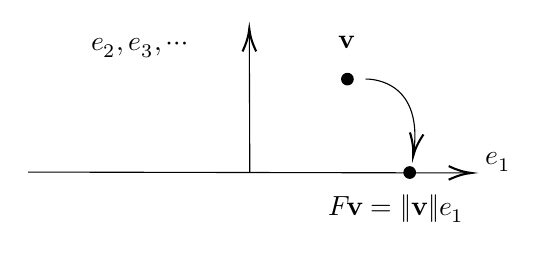
\begin{tikzpicture}[x=0.75pt,y=0.75pt,yscale=-1,xscale=1]
%uncomment if require: \path (0,300); %set diagram left start at 0, and has height of 300

%Straight Lines [id:da348568157801016] 
\draw    (176,191) -- (387.5,191.42) ;
\draw [shift={(389.5,191.43)}, rotate = 180.12] [color={rgb, 255:red, 0; green, 0; blue, 0 }  ][line width=0.75]    (10.93,-3.29) .. controls (6.95,-1.4) and (3.31,-0.3) .. (0,0) .. controls (3.31,0.3) and (6.95,1.4) .. (10.93,3.29)   ;
%Straight Lines [id:da4079481249226018] 
\draw    (282.75,191.21) -- (282.51,123.93) ;
\draw [shift={(282.5,121.93)}, rotate = 449.79] [color={rgb, 255:red, 0; green, 0; blue, 0 }  ][line width=0.75]    (10.93,-3.29) .. controls (6.95,-1.4) and (3.31,-0.3) .. (0,0) .. controls (3.31,0.3) and (6.95,1.4) .. (10.93,3.29)   ;
%Shape: Circle [id:dp39340928707014067] 
\draw  [color={rgb, 255:red, 0; green, 0; blue, 0 }  ,draw opacity=1 ][fill={rgb, 255:red, 1; green, 1; blue, 1 }  ,fill opacity=1 ] (327,146.21) .. controls (327,144.68) and (328.25,143.43) .. (329.79,143.43) .. controls (331.32,143.43) and (332.57,144.68) .. (332.57,146.21) .. controls (332.57,147.75) and (331.32,149) .. (329.79,149) .. controls (328.25,149) and (327,147.75) .. (327,146.21) -- cycle ;
%Shape: Circle [id:dp3909060606451584] 
\draw  [color={rgb, 255:red, 0; green, 0; blue, 0 }  ,draw opacity=1 ][fill={rgb, 255:red, 1; green, 1; blue, 1 }  ,fill opacity=1 ] (357,191.21) .. controls (357,189.68) and (358.25,188.43) .. (359.79,188.43) .. controls (361.32,188.43) and (362.57,189.68) .. (362.57,191.21) .. controls (362.57,192.75) and (361.32,194) .. (359.79,194) .. controls (358.25,194) and (357,192.75) .. (357,191.21) -- cycle ;
%Curve Lines [id:da32886361031606026] 
\draw    (338.5,146.2) .. controls (337.52,146.2) and (366.61,144.26) .. (361.75,181.47) ;
\draw [shift={(361.5,183.2)}, rotate = 278.75] [color={rgb, 255:red, 0; green, 0; blue, 0 }  ][line width=0.75]    (10.93,-3.29) .. controls (6.95,-1.4) and (3.31,-0.3) .. (0,0) .. controls (3.31,0.3) and (6.95,1.4) .. (10.93,3.29)   ;

% Text Node
\draw (395,180.4) node [anchor=north west][inner sep=0.75pt]    {$e_{1}$};
% Text Node
\draw (205,125.4) node [anchor=north west][inner sep=0.75pt]    {$e_{2} ,e_{3} ,\cdots $};
% Text Node
\draw (324,124.4) node [anchor=north west][inner sep=0.75pt]    {$\mathbf{v}$};
% Text Node
\draw (319.5,200.6) node [anchor=north west][inner sep=0.75pt]    {$F\mathbf{v} =\| \mathbf{v} \| e_{1}$};

\end{tikzpicture}

\end{center}

Suppose we define \(\mathbf{w} = \|\mathbf{v}\| e_1 - \mathbf{v}\),
then, we have \(\mathbf{w}\) is orthogonal to the hyperplane \(\Sigma\).
With that in mind, we see that the image of the projector defined by
\[P' = \frac{\mathbf{w} \mathbf{w}^T}{\mathbf{w}^T \mathbf{w}}\] is the
plane orthogonal to \(\Sigma\). Hence, the projector to \(\Sigma\) is
simply the complementary projector to \(P'\), \(P = I - P'\).

\begin{center}

\tikzset{every picture/.style={line width=0.75pt}} %set default line width to 0.75pt        

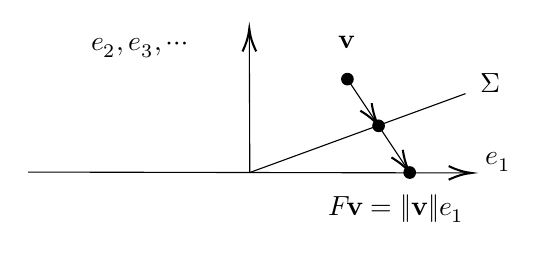
\begin{tikzpicture}[x=0.75pt,y=0.75pt,yscale=-1,xscale=1]
%uncomment if require: \path (0,300); %set diagram left start at 0, and has height of 300

%Straight Lines [id:da348568157801016] 
\draw    (176,191) -- (387.5,191.42) ;
\draw [shift={(389.5,191.43)}, rotate = 180.12] [color={rgb, 255:red, 0; green, 0; blue, 0 }  ][line width=0.75]    (10.93,-3.29) .. controls (6.95,-1.4) and (3.31,-0.3) .. (0,0) .. controls (3.31,0.3) and (6.95,1.4) .. (10.93,3.29)   ;
%Straight Lines [id:da4079481249226018] 
\draw    (282.75,191.21) -- (282.51,123.93) ;
\draw [shift={(282.5,121.93)}, rotate = 449.79] [color={rgb, 255:red, 0; green, 0; blue, 0 }  ][line width=0.75]    (10.93,-3.29) .. controls (6.95,-1.4) and (3.31,-0.3) .. (0,0) .. controls (3.31,0.3) and (6.95,1.4) .. (10.93,3.29)   ;
%Shape: Circle [id:dp39340928707014067] 
\draw  [color={rgb, 255:red, 0; green, 0; blue, 0 }  ,draw opacity=1 ][fill={rgb, 255:red, 1; green, 1; blue, 1 }  ,fill opacity=1 ] (327,146.21) .. controls (327,144.68) and (328.25,143.43) .. (329.79,143.43) .. controls (331.32,143.43) and (332.57,144.68) .. (332.57,146.21) .. controls (332.57,147.75) and (331.32,149) .. (329.79,149) .. controls (328.25,149) and (327,147.75) .. (327,146.21) -- cycle ;
%Shape: Circle [id:dp3909060606451584] 
\draw  [color={rgb, 255:red, 0; green, 0; blue, 0 }  ,draw opacity=1 ][fill={rgb, 255:red, 1; green, 1; blue, 1 }  ,fill opacity=1 ] (357,191.21) .. controls (357,189.68) and (358.25,188.43) .. (359.79,188.43) .. controls (361.32,188.43) and (362.57,189.68) .. (362.57,191.21) .. controls (362.57,192.75) and (361.32,194) .. (359.79,194) .. controls (358.25,194) and (357,192.75) .. (357,191.21) -- cycle ;
%Straight Lines [id:da0874932667980326] 
\draw    (282.75,191.21) -- (386.7,153.2) ;
%Shape: Circle [id:dp34536838295442895] 
\draw  [color={rgb, 255:red, 0; green, 0; blue, 0 }  ,draw opacity=1 ][fill={rgb, 255:red, 1; green, 1; blue, 1 }  ,fill opacity=1 ] (342,168.71) .. controls (342,167.18) and (343.25,165.93) .. (344.79,165.93) .. controls (346.32,165.93) and (347.57,167.18) .. (347.57,168.71) .. controls (347.57,170.25) and (346.32,171.5) .. (344.79,171.5) .. controls (343.25,171.5) and (342,170.25) .. (342,168.71) -- cycle ;
%Straight Lines [id:da12375469389911808] 
\draw    (329.79,146.21) -- (343.68,167.05) ;
\draw [shift={(344.79,168.71)}, rotate = 236.31] [color={rgb, 255:red, 0; green, 0; blue, 0 }  ][line width=0.75]    (10.93,-3.29) .. controls (6.95,-1.4) and (3.31,-0.3) .. (0,0) .. controls (3.31,0.3) and (6.95,1.4) .. (10.93,3.29)   ;
%Straight Lines [id:da7562346398871844] 
\draw    (344.79,168.71) -- (358.68,189.55) ;
\draw [shift={(359.79,191.21)}, rotate = 236.31] [color={rgb, 255:red, 0; green, 0; blue, 0 }  ][line width=0.75]    (10.93,-3.29) .. controls (6.95,-1.4) and (3.31,-0.3) .. (0,0) .. controls (3.31,0.3) and (6.95,1.4) .. (10.93,3.29)   ;

% Text Node
\draw (395,180.4) node [anchor=north west][inner sep=0.75pt]    {$e_{1}$};
% Text Node
\draw (205,125.4) node [anchor=north west][inner sep=0.75pt]    {$e_{2} ,e_{3} ,\cdots $};
% Text Node
\draw (324,124.4) node [anchor=north west][inner sep=0.75pt]    {$\mathbf{v}$};
% Text Node
\draw (319.5,200.6) node [anchor=north west][inner sep=0.75pt]    {$F\mathbf{v} =\| \mathbf{v} \| e_{1}$};
% Text Node
\draw (392.7,142.4) node [anchor=north west][inner sep=0.75pt]    {$\Sigma $};

\end{tikzpicture}

\end{center}

However, we do not wish to project into \(\Sigma\) but to reflect around
it. Thus, to reflect around \(\Sigma\) we projecting twice as the
distance in the same direction. This results in the desired Householder
reflector,
\[F = I - 2 \frac{\mathbf{w} \mathbf{w}^T}{\mathbf{w}^T \mathbf{w}},\]
where \(\mathbf{w} = \|\mathbf{v}\| e_1 - \mathbf{v}\).

We note that this is not the only possible reflection as we may reflect
around the hyperplane \(\Sigma_2\) as demonstrated in the figure below.

\begin{center}
  \tikzset{every picture/.style={line width=0.75pt}} %set default line width to 0.75pt        

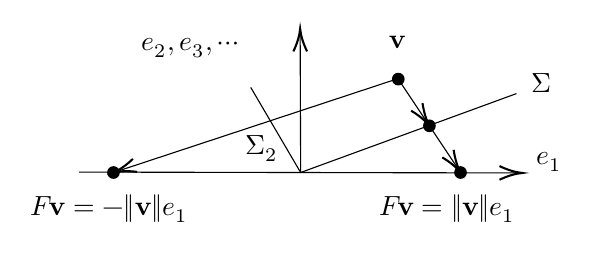
\begin{tikzpicture}[x=0.75pt,y=0.75pt,yscale=-1,xscale=1]
%uncomment if require: \path (0,300); %set diagram left start at 0, and has height of 300

%Straight Lines [id:da348568157801016] 
\draw    (176,191) -- (387.5,191.42) ;
\draw [shift={(389.5,191.43)}, rotate = 180.12] [color={rgb, 255:red, 0; green, 0; blue, 0 }  ][line width=0.75]    (10.93,-3.29) .. controls (6.95,-1.4) and (3.31,-0.3) .. (0,0) .. controls (3.31,0.3) and (6.95,1.4) .. (10.93,3.29)   ;
%Straight Lines [id:da4079481249226018] 
\draw    (282.75,191.21) -- (282.51,123.93) ;
\draw [shift={(282.5,121.93)}, rotate = 449.79] [color={rgb, 255:red, 0; green, 0; blue, 0 }  ][line width=0.75]    (10.93,-3.29) .. controls (6.95,-1.4) and (3.31,-0.3) .. (0,0) .. controls (3.31,0.3) and (6.95,1.4) .. (10.93,3.29)   ;
%Shape: Circle [id:dp39340928707014067] 
\draw  [color={rgb, 255:red, 0; green, 0; blue, 0 }  ,draw opacity=1 ][fill={rgb, 255:red, 1; green, 1; blue, 1 }  ,fill opacity=1 ] (327,146.21) .. controls (327,144.68) and (328.25,143.43) .. (329.79,143.43) .. controls (331.32,143.43) and (332.57,144.68) .. (332.57,146.21) .. controls (332.57,147.75) and (331.32,149) .. (329.79,149) .. controls (328.25,149) and (327,147.75) .. (327,146.21) -- cycle ;
%Shape: Circle [id:dp3909060606451584] 
\draw  [color={rgb, 255:red, 0; green, 0; blue, 0 }  ,draw opacity=1 ][fill={rgb, 255:red, 1; green, 1; blue, 1 }  ,fill opacity=1 ] (357,191.21) .. controls (357,189.68) and (358.25,188.43) .. (359.79,188.43) .. controls (361.32,188.43) and (362.57,189.68) .. (362.57,191.21) .. controls (362.57,192.75) and (361.32,194) .. (359.79,194) .. controls (358.25,194) and (357,192.75) .. (357,191.21) -- cycle ;
%Straight Lines [id:da0874932667980326] 
\draw    (282.75,191.21) -- (386.7,153.2) ;
%Shape: Circle [id:dp34536838295442895] 
\draw  [color={rgb, 255:red, 0; green, 0; blue, 0 }  ,draw opacity=1 ][fill={rgb, 255:red, 1; green, 1; blue, 1 }  ,fill opacity=1 ] (342,168.71) .. controls (342,167.18) and (343.25,165.93) .. (344.79,165.93) .. controls (346.32,165.93) and (347.57,167.18) .. (347.57,168.71) .. controls (347.57,170.25) and (346.32,171.5) .. (344.79,171.5) .. controls (343.25,171.5) and (342,170.25) .. (342,168.71) -- cycle ;
%Straight Lines [id:da12375469389911808] 
\draw    (329.79,146.21) -- (343.68,167.05) ;
\draw [shift={(344.79,168.71)}, rotate = 236.31] [color={rgb, 255:red, 0; green, 0; blue, 0 }  ][line width=0.75]    (10.93,-3.29) .. controls (6.95,-1.4) and (3.31,-0.3) .. (0,0) .. controls (3.31,0.3) and (6.95,1.4) .. (10.93,3.29)   ;
%Straight Lines [id:da7562346398871844] 
\draw    (344.79,168.71) -- (358.68,189.55) ;
\draw [shift={(359.79,191.21)}, rotate = 236.31] [color={rgb, 255:red, 0; green, 0; blue, 0 }  ][line width=0.75]    (10.93,-3.29) .. controls (6.95,-1.4) and (3.31,-0.3) .. (0,0) .. controls (3.31,0.3) and (6.95,1.4) .. (10.93,3.29)   ;
%Straight Lines [id:da8768367612062469] 
\draw    (258.7,150.2) -- (282.75,191.21) ;
%Straight Lines [id:da7861570902013968] 
\draw    (328.87,146.23) -- (194.47,190.59) ;
\draw [shift={(192.57,191.21)}, rotate = 341.73] [color={rgb, 255:red, 0; green, 0; blue, 0 }  ][line width=0.75]    (10.93,-3.29) .. controls (6.95,-1.4) and (3.31,-0.3) .. (0,0) .. controls (3.31,0.3) and (6.95,1.4) .. (10.93,3.29)   ;
%Shape: Circle [id:dp7818054470996165] 
\draw  [color={rgb, 255:red, 0; green, 0; blue, 0 }  ,draw opacity=1 ][fill={rgb, 255:red, 1; green, 1; blue, 1 }  ,fill opacity=1 ] (189.79,191.21) .. controls (189.79,189.68) and (191.03,188.43) .. (192.57,188.43) .. controls (194.11,188.43) and (195.36,189.68) .. (195.36,191.21) .. controls (195.36,192.75) and (194.11,194) .. (192.57,194) .. controls (191.03,194) and (189.79,192.75) .. (189.79,191.21) -- cycle ;

% Text Node
\draw (395,180.4) node [anchor=north west][inner sep=0.75pt]    {$e_{1}$};
% Text Node
\draw (205,125.4) node [anchor=north west][inner sep=0.75pt]    {$e_{2} ,e_{3} ,\cdots $};
% Text Node
\draw (324,124.4) node [anchor=north west][inner sep=0.75pt]    {$\mathbf{v}$};
% Text Node
\draw (319.5,200.6) node [anchor=north west][inner sep=0.75pt]    {$F\mathbf{v} =\| \mathbf{v} \| e_{1}$};
% Text Node
\draw (392.7,142.4) node [anchor=north west][inner sep=0.75pt]    {$\Sigma $};
% Text Node
\draw (254.7,172.4) node [anchor=north west][inner sep=0.75pt]    {$\Sigma _{2}$};
% Text Node
\draw (151.5,200.6) node [anchor=north west][inner sep=0.75pt]    {$F\mathbf{v} =-\| \mathbf{v} \| e_{1}$};

\end{tikzpicture}
\end{center}

Mathematically, the choice does not matter as both transformations
results in the vector with only components in \(e_1\), however, as often
times in numerical analysis, we need to consider the computers in
computing these values. Indeed, by considering that if we reflect by a
plane which is almost parallel to the \(e_1\)-axis, the computer is
required to work with large numbers and so, could possible encounter
cancellation errors. Thus, it is usually better to choose the shallow
plane to reflect around.

With that, we arrive at the Householder-based QR-decomposition.

\begin{alg}[Householder-based QR-decomposition]
  If \(A \in M_{m \times n}(\mathbb{R})\) be the matrix we are decomposing, then,
  for \(k = 1,\cdots n\), we define 
  \begin{itemize}
    \item \(\mathbf{x} := A_{k : m, k}\) that is, the \(k\) to \(m\)-th 
      entry of the \(k\)-th row of \(A\);
    \item \(\mathbf{v}_k := \text{sign}(x_1) \| \mathbf{x} \|e_1 + \mathbf{x}\);
    \item \(\mathbf{v}_k := \mathbf{v}_k / \| \mathbf{v}_k \|\);
    \item \(A_{k:m, k:n} := A_{k:m, k:n} - 2\mathbf{v}_k(\mathbf{v}_k^T A_{k:m, k:n})\).
  \end{itemize}

\end{alg}

Thus, by successively applying the Householder reflection, we achieve
the QR-decomposition.

\begin{center}
\tikzset{every picture/.style={line width=0.75pt}} %set default line width to 0.75pt        

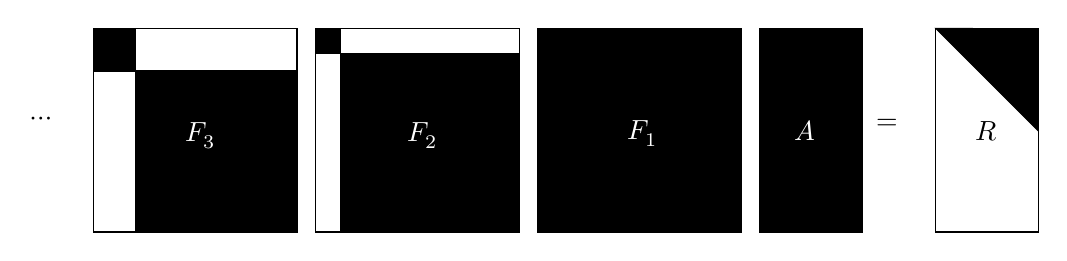
\begin{tikzpicture}[x=0.75pt,y=0.75pt,yscale=-1,xscale=1]
%uncomment if require: \path (0,300); %set diagram left start at 0, and has height of 300

%Shape: Rectangle [id:dp5208320846231114] 
\draw  [fill={rgb, 255:red, 0; green, 0; blue, 0 }  ,fill opacity=1 ] (492.5,61.08) -- (541.94,61.08) -- (541.94,159.2) -- (492.5,159.2) -- cycle ;
%Shape: Rectangle [id:dp8949758616800922] 
\draw  [fill={rgb, 255:red, 255; green, 255; blue, 255 }  ,fill opacity=1 ] (577.26,61.08) -- (626.7,61.08) -- (626.7,159.2) -- (577.26,159.2) -- cycle ;
%Shape: Right Triangle [id:dp06276901677064406] 
\draw  [fill={rgb, 255:red, 0; green, 0; blue, 0 }  ,fill opacity=1 ] (626.43,110.24) -- (577.26,61.08) -- (626.7,61.29) -- cycle ;
%Shape: Square [id:dp8062846556416521] 
\draw  [fill={rgb, 255:red, 0; green, 0; blue, 0 }  ,fill opacity=1 ] (385.3,61) -- (483.5,61) -- (483.5,159.2) -- (385.3,159.2) -- cycle ;
%Shape: Square [id:dp5607518636916182] 
\draw  [fill={rgb, 255:red, 0; green, 0; blue, 0 }  ,fill opacity=1 ] (278.3,61) -- (376.5,61) -- (376.5,159.2) -- (278.3,159.2) -- cycle ;
%Shape: Rectangle [id:dp6236451543115944] 
\draw  [fill={rgb, 255:red, 255; green, 255; blue, 255 }  ,fill opacity=1 ] (290.5,61) -- (376.5,61) -- (376.5,73.2) -- (290.5,73.2) -- cycle ;
%Shape: Rectangle [id:dp5004590223579148] 
\draw  [fill={rgb, 255:red, 255; green, 255; blue, 255 }  ,fill opacity=1 ] (290.5,73.2) -- (290.5,159.2) -- (278.3,159.2) -- (278.3,73.2) -- cycle ;
%Shape: Square [id:dp8828339790523514] 
\draw  [fill={rgb, 255:red, 0; green, 0; blue, 0 }  ,fill opacity=1 ] (171.3,61) -- (269.5,61) -- (269.5,159.2) -- (171.3,159.2) -- cycle ;
%Shape: Rectangle [id:dp763626399594441] 
\draw  [fill={rgb, 255:red, 255; green, 255; blue, 255 }  ,fill opacity=1 ] (191.5,61) -- (269.5,61) -- (269.5,81.6) -- (191.5,81.6) -- cycle ;
%Shape: Rectangle [id:dp417925154559905] 
\draw  [fill={rgb, 255:red, 255; green, 255; blue, 255 }  ,fill opacity=1 ] (191.5,81.6) -- (191.5,159.2) -- (171.3,159.2) -- (171.3,81.6) -- cycle ;

% Text Node
\draw (507.93,104.31) node [anchor=north west][inner sep=0.75pt]  [color={rgb, 255:red, 255; green, 255; blue, 255 }  ,opacity=1 ]  {$A$};
% Text Node
\draw (547.61,103.73) node [anchor=north west][inner sep=0.75pt]    {$=$};
% Text Node
\draw (595.1,104.68) node [anchor=north west][inner sep=0.75pt]    {$R$};
% Text Node
\draw (427.5,104.4) node [anchor=north west][inner sep=0.75pt]  [color={rgb, 255:red, 255; green, 255; blue, 255 }  ,opacity=1 ]  {$F_{1}$};
% Text Node
\draw (321.5,105.4) node [anchor=north west][inner sep=0.75pt]  [color={rgb, 255:red, 255; green, 255; blue, 255 }  ,opacity=1 ]  {$F_{2}$};
% Text Node
\draw (214.5,105.4) node [anchor=north west][inner sep=0.75pt]  [color={rgb, 255:red, 255; green, 255; blue, 255 }  ,opacity=1 ]  {$F_{3}$};
% Text Node
\draw (140,102.4) node [anchor=north west][inner sep=0.75pt]    {$\cdots $};

\end{tikzpicture}
\end{center}

By recalling the Gram-Schmdit QR-decomposition where we can consider the
algorithm as sequentially applying upper triangular matrices to \(A\)
until it becomes orthogonal, so, \[A R_1 R_2 \cdots R_n = Q,\] and thus,
\(\prod R_i = R^{-1}\). With that, we can describe the Gram-Schmidt
process as a \emph{triangular orthogonalisation} while, on the other
hand, the Householder algorithm is a \emph{orthogonal
triangularisation}. Indeed, the two process are not equivalent and
consequentially, the resulting QR-decompositions are different. We
notice that the Gram-Schmidt procedure results in \(R\) being square
while \(Q\) rectangular, that is, it yields the \emph{reduced form} of
the QR-decomposition. The Householder decomposition, on the other hand,
results in \(Q\) being square while \(R\) being rectangular. This is
refereed as the \emph{full form} of the QR-decomposition and by noticing
that the additional parts of \(Q\) are multiplied by 0, we have that the
full form provides us with information about the null-space of \(A\).

\hypertarget{least-square-problems}{%
\subsection{Least Square Problems}\label{least-square-problems}}

Least square problems are often found in data fitting, statistics,
computational modelling and many other fields, e.g.~minimising the mean
square error for an estimator. Least square problems are also
significant historically as they constitute one of the earliest problems
formulated in matrix form by Gauss.

A least square problem aims at the solution of an overdetermined system
of equations, that is, we have the linear system of the form
\[A\mathbf{x} = \mathbf{b},\] where \(A \in \mathbb{R}^{m \times n}\)
for some \(m > n\).

In general, we do not have a solution to this problem, however, we may
minimise the 2-norm of the residual given by
\[\mathbf{r} = \mathbf{b} - A\mathbf{x}.\] Straight away, we see that,
since we have more equations than unknowns, there exists a solution to
our linear system of equations if and only if
\(\mathbf{b} \in \text{Im}A\) and in this case, the residual
\(\mathbf{r} = 0\). On the other hand, if
\(\mathbf{b} \notin \text{Im}A\), then we are tasked with finding
\(\mathbf{x} \in \mathbb{R}^n\) such that
\[\mathbf{x} = \text{argmin}_\mathbf{x} \| \mathbf{b} - A\mathbf{x} \|_2,\]
where we uses the 2-norm as its derivative yields a linear system, and
so, can be solved using standard linear algebra techniques.

Geometrically, we see that the residual vector \(\mathbf{r}\) is
orthogonal to the image of \(A\) whenever it is minimized, so we have
the restriction that, for all \(\mathbf{v} \in \mathbb{R}^n\),
\[0 = \langle A\mathbf{v}, \mathbf{r} \rangle = \mathbf{v}^TA^T\mathbf{r},\]
and so, \(A^T \mathbf{r} = 0\). Indeed, by considering that, for all
\(\mathbf{x} \in \mathbb{R}^n\), \(A\mathbf{x}\) is the orthogonal
projection \(P\) of \(\mathbf{b}\) onto the image of \(A\), we have
\(A\mathbf{x} = P\mathbf{b}\). So, the least square problem is rephrased
such that we need to find such a projection \(P\).

We shall look at two methods for finding such a projection the first of
which follows straight away when we impose the orthogonality condition.
As we require the residual to be orthogonal to the image, we have
\[A^T(\mathbf{b} - A\mathbf{x}) = 0\] and so,
\[A^TA \mathbf{x} = A^T \mathbf{b}.\] This equation is known as the
normal equation, and with this, we see that, since \(A^T A\) is
nonsingular if and only if \(A\) has full rank, the least square problem
has a unique solution \(\mathbf{x}\) if and only if \(A\) has full rank.
Thus, if \(A\) has full rank, we have
\[\mathbf{x} = (A^T A)^{-1} A^T \mathbf{b},\] and in some sense, the
triple product \((A^T A)^{-1} A^T\) is a kind of (pseudo)-inverse.

\begin{definition}[Pseudo-inverse]
  Given a matrix \(A \in \mathbb{R}^{n \times m}\), if \(A\) has full rank then, 
  the pseudo-inverse of \(A\) is 
  \[A^+ = (A^T A)^{-1} A^T.\]
\end{definition}

This naive approach to the least square problem can produce
ill-conditioned matrices and is expensive since it required the
computation of a inverse and therefore is rarely used to solve least
square problems. A better approach is to use the QR-decomposition.
Rather than orthogonalising the residual onto the image of \(A\), we
instead form the projector directly.

Suppose we have decomposed the matrix \(A\) in to \(A = QR\), and let us
define \(P = Q Q^T\). Then, by considering
\(P\mathbf{b} = QQ^T \mathbf{b}\), we have
\[QR \mathbf{x} = QQ^T \mathbf{b},\] and so, by multiplying both side by
\(Q^T\), by the orthogonality of \(Q\), we have
\(R\mathbf{x} = Q^T\mathbf{b}\). Thus, by backwards substitution, we may
find \(\mathbf{x}\) given \(R\) is full rank (which is true if and only
if \(A\) is full rank). Furthermore, by comparing the two methods, since
the solution is unique (provided \(A\) if full rank), we find
\[A^+ = R^{-1} Q^T,\] and \(\mathbf{x} = A^+\mathbf{b}\).

We note that in the second method above, we have used the reduced form
of the QR-decomposition. Using the full form instead, we may obtain more
information about the residual of the least square problem. Suppose we
decompose \(A = QR\) where \(Q \in \mathbb{R}^{m \times m}\) and
\(R \in \mathbb{R}^{m \times n}\). As before, we project \(\mathbf{b}\)
onto the image of \(A\) by \(Q^T\). However, since the full form also
represents the kernel of \(A\), we can decompose \(Q^T\mathbf{b}\),
\[Q^T \mathbf{b} = \alpha + \beta =  
\begin{pmatrix}
  (Q^T \mathbf{b})_1 \\ \vdots\\ (Q^T \mathbf{b})_n\\ 0\\ \vdots\\ 0
\end{pmatrix} + 
\begin{pmatrix}
  0\\ \vdots\\ 0\\ (Q^T \mathbf{b})_{n + 1} \\ \vdots\\ (Q^T \mathbf{b})_m
\end{pmatrix},\] where \(Q^T\beta \in \ker A\) and
\(Q^T\alpha \in \text{Im}\hspace{1mm} A\). Consider the case when
\(\beta = 0\). Indeed, if \(\beta = 0\) then we have,
\[R\mathbf{x} = Q^TQR \mathbf{x} = Q^TA\mathbf{x} = Q^T\mathbf{b} = \alpha.\]
So, \(0 = R\mathbf{x} - Q^T\mathbf{b}\) and hence,
\[0 = QR\mathbf{x} - QQ^T\mathbf{b} = A\mathbf{x} - \mathbf{b}.\] We
note that in the full QR-decomposition, \(Q\) is a square orthogonal
matrix and so \(Q Q^T = I\). Now, if \(\beta \neq 0\), we have
\(R\mathbf{x} = Q^T\mathbf{b}\) is a inconsistent system. Since
\(Q^T\alpha \in \text{Im}\hspace{1mm} A\), we have
\(\alpha \in \text{Im}\hspace{1mm} R\) and so, there exists some
\(\mathbf{x}^* \in \mathbb{R}^n\) such that \(R\mathbf{x}^* = \alpha\).
This is in fact the solution to the least square problem since
\[\begin{split}
  \|A\mathbf{x} - b\|^2 & = \|Q^T(A \mathbf{x} - b)\|^2\\
    & = \|R\mathbf{x} - (\alpha + \beta)\|^2\\
    & = \langle (R\mathbf{x} - \alpha) - \beta, (R\mathbf{x} - \alpha) - \beta \rangle\\
    & = \|R\mathbf{x} - \alpha\|^2 - 2\langle R\mathbf{x} - \alpha, \beta \rangle + \|\beta\|^2.
\end{split}\] Thus, by considering
\(\langle R\mathbf{x} - \alpha, \beta \rangle = \langle R(\mathbf{x} - \mathbf{x}^*), \beta \rangle = 0\)
we have
\(\|A\mathbf{x} - b\|^2 = \|R\mathbf{x} - \alpha\|^2 + \|\beta\|^2 = \|\beta\|^2\)
whenever \(x = x^*\). So, \(x^*\) is the solution and \(\|\beta\|\) is
the norm of the residual.

\hypertarget{lu-decomposition}{%
\subsection{LU-Decomposition}\label{lu-decomposition}}

As we have seen, the QR-decomposition provides us with a method for
solving a system of equation with more equations than unknowns and this
decomposition can also be used when ever we would like to solve a system
with equal number of equations as unknowns. However, this problem can be
solved more efficiently through the LU-decomposition.

Similar to the QR-decomposition, the LU-decompostion shall manipulate
the matrix column by column in order to reduce the matrix to
upper-triangular form. In contrast to the Householder QR-decomposition
however, we shall achieve this through a sequence of lower-triangular
matrices, i.e.~ \[L_{m - 1} \cdots L_2 L_1 A = U,\] where
\(A \in \mathbb{R}^{m \times n}\), \(U\) upper-triangular and
\((\prod L_i)^{-1}\) lower-triangular.

This decomposition is helpful in solving the linear equation
\(A\mathbf{x} = \mathbf{b}\) since if \(A = LU\), we have
\(\mathbf{b} = L (U\mathbf{x}) = L\mathbf{y}\). Thus, by using forward
substitution, we can solve \(\mathbf{y}\) resulting in the system
\(U\mathbf{x} = \mathbf{y}\) which can be solved using backwards
substitution.

Consider for each step, we require the operator \(L_k\) to turn a
general vector into a vector with 0 below the \(k\)-th entries, i.e.
\[\begin{pmatrix}
  x_{1, k} \\ \vdots \\ x_{k, k} \\ x_{k + 1, k} \\ \vdots \\ x_{m, k}
  \end{pmatrix} 
  \xrightarrow[]{L_k} 
  \begin{pmatrix}
  x_{1, k} \\ \vdots \\ x_{k, k} \\ 0 \\ \vdots \\ 0
  \end{pmatrix},\] and so, we see that \[L_k = 
\begin{pmatrix}
  1 & & & & & \\
  & \ddots & & & & \\
  & & 1 & & & \\
  & & -l_{k + 1, k} & 1 & & \\
  & & \vdots & & \ddots & \\
  & & -l_{m, k} & & & 1
\end{pmatrix},\] where \(l_{j, k} = x_{j, k} / x_{k, k}\) for
\(k < j \le m\). However, this algorithm as it stands is numerically
unstable. Indeed, if there exists a \(0\) on the diagonal then the
algorithm will need to divide by zero! To combat this, we will introduce
an additional step called \emph{partial pivoting}.

Consider instead, when acting on the \(k\)-th column of \(A\), we denote
\(i\) for the entry of \(A_{k:m, k}\) with maximum absolute value. Then,
by multiplying by a permutation matrix \(P\), we may swap the \(i\)-th
entry with the \(k\)-th entry of \(A_{k:m, k}\) and we may proceed with
the standard LU-step. Thus, the full decomposition becomes
\[L_{m - 1}P_{m -1} \cdots L_2 P_2 L_1 P_1 A = U.\] Now, (as seen on the
problem sheet) we have, \[L_{m - 1}P_{m -1} \cdots L_2 P_2 L_1 P_1 
  = L_{m - 1}' \cdots L_2' L_1' P_{m - 1} \cdots P_2 P_1,\] where
\(L_i'\) are also lower-triangular matrices. Thus, this modified
procedure results in the linear system \[PA = LU,\] where
\(P = \prod P_i\) is a permutation matrix. In other words, to achieve
the LU-decomposition with partial pivoting all we have to do is to
permute the rows of \(A\) before hand such that for each \(k\), the
maximum entry of \(A_{k:m, k}\) is swapped with \(A_{k, k}\) and then
proceeding as usual.

\hypertarget{cholesky-decomposition}{%
\subsection{Cholesky Decomposition}\label{cholesky-decomposition}}

The Cholesky decomposition is a decomposition that applies to a narrow
but important type of matrices -- symmetric, positive definite matrices.

\begin{definition}[Symmetric, Positive Definite Matrix]
  A matrix \(A\) is symmetric and positive definite if \(A^T = A\) and 
  for all \(\mathbf{x}\), \(\mathbf{x}^T A\mathbf{x} > 0\).
\end{definition}

Equivalently, we see that symmetric positive definite matrices are
matrices whose induced bilinear form
\(\langle \cdot, \cdot \rangle_A :  (\mathbf{x}, \mathbf{y}) \mapsto \mathbf{x}^T A\mathbf{y}\)
is symmetric and positive definite.

Symmetric positive definite matrices arise in many applications such as
covariance matrices in statistics, as kernels in machine learning and as
diffusion tensors in medical imaging and weighted norms, etc.

The Cholesky decomposition can be though of as a symmetric
LU-decomposition, applying a LU-step from the left and right while
maintaining the symmetry of the resulting matrix. Starting with a
symmetric, positive definite matrix \(A\) and we write
\[A = \begin{pmatrix}
  a_{11} & \mathbf{w}^T\\
  \mathbf{w} & K
  \end{pmatrix}\] assuming \(a_{11} > 0\). Then, by defining
\[R_1^T := \begin{pmatrix}
  \sqrt{a_{11}} & 0\\
  \mathbf{w} / \sqrt{a_{11}} & I
  \end{pmatrix}, \hspace{2mm} A^{(1)} := 
  \begin{pmatrix}
    1 & 0\\
    0 & K - \mathbf{w}\mathbf{w}^T / a_{11}
  \end{pmatrix}\] by multiplying \(A^{(1)}\) with \(R_1^T\) and \(R_1\)
on each side, we obtain \[R_1^T A^{(1)} R_1 = 
  \begin{pmatrix}
  \sqrt{a_{11}} & 0\\
  \mathbf{w} / \sqrt{a_{11}} & I
  \end{pmatrix}
  \begin{pmatrix}
    1 & 0\\
    0 & K - \mathbf{w}\mathbf{w}^T / a_{11}
  \end{pmatrix}
  \begin{pmatrix}
  \sqrt{a_{11}} & \mathbf{w}^T / \sqrt{a_{11}}\\
  0 & I
  \end{pmatrix}
  = 
  \begin{pmatrix}
  a_{11} & \mathbf{w}^T\\
  \mathbf{w} & K
  \end{pmatrix} = A.\] Now, by induction, we find that
\(K - \mathbf{w}\mathbf{w}^T / a_{11}\) is also a symmetric, positive
definite matrix, and so we can find \(R_2'\) and \(A^{(2)*}\), such that
\(R_2'^T A^{(2)*} R_2' = K - \mathbf{w}\mathbf{w}^T / a_{11}\) and so,
by letting \(R_2 = 1 \oplus R_2'\) and \(A^{(2)} = 1 \oplus A^{(2)*}\),
we have \(R_2^T A^{(2)} R^2 = A^{(1)}\). Hence, by repeatedly applying
the process, we have
\[A = R_1^T R_2^T \cdots R_m^T I R_m \cdots R_2 R_1.\] So, by letting
\(R := R_m \cdots R_2 R_1\), we have \(A = R^T R\) where \(R\) is upper
triangular.

Note that we assumed the upper-left element of each submatrix is
positive. This must be true for a positive definite matrix since if
\([A]_{11} = a_{11} < 0\), then \(e_1^T A e_1 = a_{11} < 0\);
contradicting positive definiteness.

Similar to the LU-decomposition, the Cholesky decomposition can be used
to solve linear systems \(A\mathbf{x} = \mathbf{b}\) where \(A\) is
symmetric, positive definite. Indeed, if \(A = R^T R\), then
\(R^T R \mathbf{x} = \mathbf{b}\) and so, we may solve for
\(R \mathbf{x}\) using a forward substitution, and then we may solve for
\(\mathbf{x}\) with a backwards substitution.

\newpage

\hypertarget{polynomials}{%
\section{Polynomials}\label{polynomials}}

\hypertarget{lagrange-interpolation}{%
\subsection{Lagrange Interpolation}\label{lagrange-interpolation}}

Interpolation is a numerical technique to formulate a continuous
representation based on discrete data points. This is applied in many
fields especially data science. Interpolation requires a basis of
functions that are tailored to the data points and we will concentrate
on the set of polynomials. This is because polynomials are particularly
practical as they can be easily differentiated and integrated, and hence
provide us with the foundations for numerically approximating
differential and integral expressions.

\begin{definition}[Polynomial Interpolation]
  Given the data points \((z_j, f_j)_{j = 0}^n\) where \(z_i \neq z_j\) for all 
  \(i \neq j\), the polynomial \(p_n \in \mathbb{P}^n\) such that for all \(j = 0, \cdots, n\), 
  \(p_n(z_j) = f_j\) is called the interpolating polynomial (or interpolant) 
  of the data set.
\end{definition}

It is not always clear that we can always find such an interpolating
polynomial for any given data sets so we shall present a proof the the
existence by constructing the interpolant.

\begin{prop}
  Given the data points \((z_j, f_j)_{j = 0}^n\) where \(z_i \neq z_j\) for all 
  \(i \neq j\), there always exists a polynomial \(p_n \in \mathbb{P}^n\) such 
  that for all \(j = 0, \cdots, n\), \(p_n(z_j) = f_j\).
\end{prop}
\proof

Define \(l_j(z) = \prod_{k = 0; k \neq j}^n \frac{z - z_k}{z_j - z_k}\)
for all \(j = 0, \cdots, n\). Then, we see \(l_j \in \mathbb{P}^n\) and
\(l_j(z_r) = \delta_{jr}\) for all \(j, r = 0, \cdots, n\). So, by
defining \[p_n(z) = \sum_{j = 0}^n f_j l_j(z),\] we see
\(p_n(z_k) = \sum_{j = 0}^n f_j l_j(z_k) = \sum_{j = 0}^n f_j \delta_{jk} = f_k\)
and so \(p_n\) is a interpolant of our data set and we call the set of
polynomials \[L := \{ l_j \mid j = 0, \cdots, n\},\] the Lagrange basis
functions. \qed

Furthermore, it turns out that our construction is unique.

\begin{prop}
  Given the data points \((z_j, f_j)_{j = 0}^n\) where \(z_i \neq z_j\) for all 
  \(i \neq j\), there always exists a \textbf{unique} polynomial \(p_n \in \mathbb{P}^n\) 
  such that for all \(j = 0, \cdots, n\), \(p_n(z_j) = f_j\).
\end{prop}
\proof

As we have already proven existence, it suffices to show uniqueness.
Suppose \(p, q \in \mathbb{P}^n\) such that \(p(z_j) = q(z_j) = f_j\)
for all \(j = 0, \cdots, n\). Then,
\((p - q)(z_j) = p(z_j) - q(z_j) = 0\) for all \(j\), that is \(z_j\)
are the roots of \(p - q\). However, as \(p, q\) have degree \(n\),
\(p - q\) can at most have degree \(n\), so if \(p - q \neq 0\), then
\(p - q\) has at most \(n\) roots. This contradicts as we found
\(n + 1\) roots, and thus \(p - q = 0\). \qed

However, while the construction of the interpolant through the Lagrange
basis is correct, it is not necessarily nice to compute since we are
required to multiple and add many terms. Instead, we ask if it is
possible to solve the system directly for the coefficients, i.e.~can we
find \(a_k\) directly such that
\[p_n(z_j) = \sum_{k = 0}^n a_k z_j^k = f_j\] for all
\(j = 0, \cdots , n\).

By writing the question as a linear system of \(n + 1\) equations, we
see that the answer becomes obvious -- \[\begin{pmatrix}
  1 & z_0 & z_0^2 & \cdots & z_0^n\\
  1 & z_1 & z_1^2 & \cdots & z_1^n\\
  \vdots & \vdots & \vdots & & \vdots\\
  1 & z_n & z_n^2 & \cdots & z_n^n
\end{pmatrix}
\begin{pmatrix}
  a_0 \\ a_1 \\ \vdots \\ a_n
\end{pmatrix}
= 
\begin{pmatrix}
  f_0 \\ f_1 \\ \vdots \\ f_n
\end{pmatrix}.\] By observing that the first matrix is simply the
Vandemonde matrix \(V\), and by assumption, we have \(z_i \neq z_j\) for
all \(i \neq j\), \(V\) is invertible and hence, \[\begin{pmatrix}
  a_0 \\ a_1 \\ \vdots \\ a_n
\end{pmatrix} = V^{-1}
\begin{pmatrix}
  f_0 \\ f_1 \\ \vdots \\ f_n
\end{pmatrix},\] solving our interpolation. Indeed, this also provide us
with uniqueness as the inverse is unique and all interpolants satisfies
this equation.

While this is mathematically correct, inverting the Vandemonde matrix
becomes difficult as \(n\) increases and so, this method is
ill-conditioned.

\hypertarget{divided-differences}{%
\subsection{Divided Differences}\label{divided-differences}}

Alternative to the Lagrange interpolation, the divided differences
method provide us with a method to find the interpolant of a data set
recursively.

Suppose we have found the interpolant
\(p_{n - 1} \in \mathbb{P}^{n - 1}\) of the data set
\((z_j, f_k)_{j = 0}^{n - 1}\) and we are asked to find the interpolant
of \((z_j, f_k)_{j = 0}^n\), given the new data point \((z_n, f_n)\). If
we are using the Lagrange interpolation method, we are required to
compute the entire Lagrange basis again, and so, we look for an
alternative construction that will make use of \(p_{n - 1}\).

Suppose there exists some \(q_n \in \mathbb{P}^n\), \(q_n(z_j) = 0\) for
all \(j = 0, \cdots, n - 1\) such that \(p_n = p_{n - 1} + q_n\). Since,
be construction \(q_n\) has roots \(z_j\) for all
\(j = 0, \cdots, n - 1\), \[q_n(z) = C\prod_{k = 0}^{n - 1}(z - z_k)\]
for some \(C\). So,
\[p_n = p_{n - 1} + C\prod_{k = 0}^{n - 1}(z - z_k).\] Evaluating both
sides at \(z_n\), we have
\[C = \frac{f_n - p_{n - 1}(z_n)}{\prod_{k = 0}^n(z_n - z_k)},\] and so,
\[p_n(z) = p_{n - 1}(z) + (f_n - p_{n - 1}(z_n))\prod_{k = 0}^n\frac{z - z_k}{z_n - z_k}.\]
Classically, the following notation for \(C\) is used
\[f[z_0, z_1, \cdots, z_n] := C\] and is called the \emph{divided
difference} of order \(n\).

We note that \(f[z_j] = f_j\) and
\(f[z_{\pi_0}, z_{\pi_1}, \cdots, z_{\pi_n}] = f[z_0, z_1, \cdots, z_n]\),
and for any data set, we have
\[f[z_0, \cdots, z_n] = \sum_{j = 0}^n\frac{f_j}{\prod_{k = 0; k \neq j}^n(z_k - z_k)}\]

The divided differences method produce a hierarchy of interpolating
polynomials, and with recursion, this method is easy to implement and
results in the interpolant
\[p_n(z) = \sum_{j = 0}^j f[z_0, \cdots, z_j] \prod_{k = 0}^{j - 1}(z - z_k)\]
and is refereed to as the \emph{Newton form} of the interpolating
polynomial.

However, while this form is rather nice, it is not necessarily obvious
the speed at which we can generate the divided differences. It turns out
that for distinct \(z_0, \cdots, z_{n + 1}\), we have
\[f[z_0, \cdots, z_{n + 1}] = \frac{f[z_0, \cdots, z_n] - f[z_1, \cdots, z_{n + 1}]}
  {z_0 - z_{n + 1}}\] (for proof see exercise), and so, we can use this
recurrence relation to generate a divided difference tableau (see
slides).

\hypertarget{orthogonal-polynomials}{%
\subsection{Orthogonal Polynomials}\label{orthogonal-polynomials}}

Orthogonal polynomials play an important role in numerical analysis.
They are key in approximation theory and feature in the solutions of
differential equations by high-order, spectral methods.

\begin{definition}
  Consider the vector space \(V = C([a, b])\) and suppose \(w : [a, b] \to \mathbb{R}^+\)
  is some weigh function such that \(w\) is integrable and 
  \(\int_a^b w(x) \dd x < \infty\). Then \(\langle \cdot, \cdot \rangle : V \times V \to \mathbb{R}\) 
  defined by 
  \[\langle f, g \rangle := \int_a^b w(x) f(x) g(x) \dd x,\]
  is an inner product on \(V\).
\end{definition}

We see that this inner product is well defined since
\[|\langle f, g \rangle| = \left| \int_a^b w f g \right| 
      \le \int_a^b |w f g| \le 
      \max_{a \le x \le b}|f(x)| \max_{a \le x \le b}|g(x)|\int_a^b w < \infty.\]
Furthermore, we easily see that it forms an inner product by checking
the axioms.

Orthogonal polynomials satisfy a three-term recurrence relation. Suppose
\(U = \mathbb{P}_n\), that is the set of polynomials of degree less than
or equal to \(n\). Furthermore, let \(\{\Phi_i\}_{i = 0}^n\) be the
canonical polynomial basis of \(U\) and we wish to consider orthogonal
monic polynomials with \(\langle p_i, p_j \rangle = 0\) whenever
\(i \neq j\).

\begin{prop}
  If \(\{p_i\}_{i = 0}^{n}\) is a sequence of monic orthogonal polynomials where 
  \(\deg p_i = i\). Then it satisfies 
  \[p_{j + i}(x) = (x - a_j) p_j(x) - b_j p_{j - 1}(x),\]
  where \(a_j = \langle xp_j, p_j \rangle / \|p_j\|^2\) and 
  \(b_j = \|p_j\|^2 / \|p_{j - 1}\|^2\) for \(j > 1\).
\end{prop}
\proof

Consider that \(\deg p_{j + 1} - xp_j = j\) since the polynomials are
monic. Then \(p_{j + 1} - xp_j \in \mathbb{P}_j\) and so there exists
\(c_k \in \mathbb{R}\) such that
\[p_{j + 1} - xp_j = \sum_{k = 0}^j c_k p_k,\] since
\(\{p_i\}_{i = 0}^j\) forms a basis of \(\mathbb{P}_j\) as orthogonal
polynomials are linearly independent.

Now, consider \[\begin{split}
    \left\langle \sum_{k = 0}^j c_k p_k, p_i \right\rangle 
      & = \langle p_{j + 1} - xp_j, p_i \rangle 
        = \langle p_{j + 1}, p_i \rangle - \langle xp_j, p_i \rangle
        = - \langle xp_j, p_i \rangle.
  \end{split}\] On the other hand,
\[\left\langle \sum_{k = 0}^j c_k p_k, p_i \right\rangle 
    = \sum_{k = 0}^j c_k \langle p_k, p_i \rangle 
    = \sum_{k = 0}^j c_k \delta_{ki} \langle p_i, p_i \rangle = c_k \|p_i\|^2, \]
so \(c_k\|p_i\|^2 = - \langle xp_j, p_i \rangle\) and hence,
\(c_k = - \langle xp_j, p_i \rangle / \|p_i\|^2\). Now, by considering
\(\langle xp_j, p_i \rangle = \langle p_j, xp_i \rangle\), we see that,
if \(xp_i \in \mathbb{P}_{j - 1}\), then it can be written as
\(\sum_l \alpha_l p_l\) and so
\(\langle p_j, xp_i \rangle = \left\langle p_j, \sum_l \alpha_l p_l \right\rangle = 0\).
Thus, the only non-vanishing \(i\) is \(i = j - 1, j\) and, hence we
have, \[p_{j + 1} = xp_j + \sum_{k = 0}^j c_k p_k = 
    xp_j + c_{j - 1}p_{j - 1} + c_j p_j = (x - a_j) p_j - b_j p_{j - 1}\]
as required. \qed

By directly checking, its not hard to see that this condition is also
sufficient and thus, we have found an exhaustive method for constructing
orthogonal monic polynomials by using the aforementioned recurrence
relation.

Let us now consider some commonly occurring inner products. In the case
that \(w = 1\) and \([a, b] = [-1, 1]\), we have the unweighted inner
production where \[\langle f, g \rangle = \int_{-1}^1 fg.\] Starting
with \(p_0(x) = 1\) and \(p_1(x) = x - a_0\) we have
\(a_0 = \langle xp_0, p_0 \rangle / \|p_0\|^2 = 0\) and so
\(p_1(x) = x\). Using the recurrence relation, we have
\(p_2(x) = x^2 - a_1 x - b_1\), and by calculating we find \(a_1 = 0\)
and \(b_1 = 1 / 3\) and so \(p_2(x) = x^2 - 1 / 3\). Repeating this
process, we can find higher terms. However, this is rather tedious and
so, it might be appropriate to write a computer programme for this.

From this, we find the orthogonal polynomials of the unweighted inner
product:
\[p_0(x) = 1,\hspace{1mm} p_1(x) = x,\hspace{1mm} p_2(x) = x^2 - \frac{1}{3},\hspace{1mm} 
  p_3(x) = x^3 - \frac{3}{5}x,\hspace{1mm} \cdots\] and these are known
as the \emph{Legendre polynomials} which are important expansion
functions for problems in spherical coordinates.

Another well-known set of orthogonal polynomials are the Chebyshev
polynomials.

\begin{definition}[Chebyshev Polynomial]
  Given \(k \in \mathbb{N}\), the \(k\)-th Chebyshev polynomial is defined to be 
  the function 
  \[T_k(x) := \cos(k \arccos (x)),\]
  for \(x \in [-1, 1]\).
\end{definition}

By computing, we find that the Chebyshev polynomials are orthogonal
under the inner product
\[\langle f, g \rangle = \int_{-1}^1 \frac{f(x)g(x)}{\sqrt{1 - x^2}} \dd x,\]
and \[\|T_k\|^2 = 
  \begin{cases}
    \pi, & k = 0;\\
    \pi / 2, & k \neq 0.
  \end{cases}\] This inner product is well defined since
\[\int_{-1}^1 \frac{1}{\sqrt{1 - x^2}} \dd x = \pi < \infty.\]
Furthermore, as the name suggests, the Chebyshev polynomials are in fact
polynomials; Indeed, we have \(T_0(x) = 1\), \(T_1(x) = x\), and for
higher \(k\), by substituting \(\theta = \arccos(x)\), we have
\(T_k(x) = \cos(k \theta)\). Thus, by using the identity
\[\cos((k + 1) \theta) + \cos((k - 1)\theta) = 2\cos(k\theta)\cos(\theta),\]
we have \[T_{k + 1}(x) + T_{k - 1}(x) = 2T_k(x)x.\] Hence, by induction,
we have \(T_k\) is a polynomial of degree \(k\) for all
\(k \in \mathbb{N}\). We note that these polynomials are not necessarily
monic.

Lastly, let us consider the domain \([a, b] = [0, \infty)\) with the
weight function \(w(x) = e^{-x}\) and the resulting polynomials are
known as the \emph{Laguerre polynomials}. Going through the recurrence
relation we find
\[L_0(x) = 1, \hspace{1mm} L_1(x) = -x + 1, \hspace{1mm} 
  L_2(x) = \frac{1}{2}(x^2 - 4 x +2), \hspace{1mm} \cdots.\] This set of
orthogonal polynomials is often applied for representing energy states
of the hydrogen atom in spherical coordinates.

\hypertarget{sturm-liouville-theory}{%
\subsection{Sturm -- Liouville Theory}\label{sturm-liouville-theory}}

In the small section we shall quickly explore other function classes
that have orthogonality properties.

Consider the real, second order linear ordinary differential equation
\[\dv{x}\left[p(x) \dv{y}{x}\right] + q(x) y = -\lambda w(x)y,\] where
\(x \in [a, b]\), \(p(x), w(x) > 0\), \(p'(x), q(x)\) continuous with
the boundary conditions \[\begin{split}
  \alpha_1 y(a) + \alpha_2 y'(a) & = 0;\\
  \beta_1 y(b) + \beta_2 y'(b) & = 0.
\end{split}\] By considering
\((\dv{x}\left[p(x) \dv{x}\right] + q(x)) / w(x)\) as an operator acting
on \(y\), we see the question becomes an eigenvalue problem for the
eigenfunction \(y\). Thus, all eigenvalues are real and simple with the
eigenfunction \(y_i\) having \(i - 1\) zeros in the interval \([a, b]\).

Furthermore, the eigenfunction form an orthogonal basis under
\(w\)-weighted inner product, i.e.~
\[\langle y_i, y_j \rangle = \int_a^b y_i(x) y_j(x) w(x) \dd x = C \delta_{ij},\]
for some \(C\) a constant.

With this, the Sturm -- Liouville problem produces classes of orthogonal
classes of functions as solutions to a differential equation. Indeed, we
may find a corresponding Sturm Liouville problem for each of our
previous examples. However, this problem does not necessarily produce
polynomials. As we have seen on the midterm project, an example of this
is the solution to the particular Sturm -- Liouville problem
\[\dv{x}\left[x \dv{y}{x}\right] + \left[x - \frac{\nu^2}{x}\right] y = 0,\]
which are the Bessel functions \(J_{\nu}(x)\) which are not polynomials.

\newpage

\hypertarget{numerical-integration}{%
\section{Numerical Integration}\label{numerical-integration}}

Numerical integration (or numerical quadrature) is concerned with with
approximation of the definite integral \[\int_a^b f(x) \dd x,\] or more
generally, the weighted definite integral \[\int_a^b f(x)w(x) \dd x,\]
for some weight function \(w\) which we assume is continuous and
positive with \[\int_a^b w(x) \dd x < \infty.\]

A method of achieving this is to replace the function \(f\) with the
\(n\)-th order interpolating polynomial. That is
\[I_n(f) = I(p_n) := \int_a^b w(x) p_n(x) \dd x,\] where \(p_n\) is the
\(n\)-th interpolating polynomial of \(f\). Thus,
\[I_n(f) = \int_a^b w(x) \sum_{k = 0}^n f(x_k)l_k(x) \dd x = 
  \sum_{k = 0}^n f(x_k) \int_a^b w(x)l_k(x) \dd x.\] Hence, by defining
the integration weights \[w_k := \int_a^b w(x) l_k(x) \dd x,\] which is
independent of \(f\), we can approximate the integral of \(f\) with
\[I_n(f) = \sum_{k = 0}^n w_k f(x_k).\] Indeed, this is exactly the same
process we have seen in the mid term project where we approximated the
derivative instead where the weights is obtained by taking the
derivative rather than the integral.

This method results in approximating the integral by trapezoids. Indeed,
by computing, we find
\[I_n(f) = \sum_{i = 0}^{n - 1}\frac{f(x_i) + f(x_{i + 1})}{2}\Delta_i,\]
where \(\Delta_i = x_{i + 1} - x_i\). Geometrically, we are partitioning
the interval \([a, b]\) into \(n - 1\) subintervals and applying the
trapezoidal rule on each. In the case where we have equispaced sampling
points, the equation simplifies to
\[I_n(f) = \frac{b - a}{n}\left(\frac{1}{2}f(a) + \sum_{i = 1}^{n - 1}f(x_i) 
  + \frac{1}{2}f(b)\right).\] We can also obtain higher-order
approximations by increasing the order of the interpolating polynomial.
Using a quadratic polynomial through \(x = a, b, \frac{a + b}{2}\), we
obtain \emph{Simpson's rule},
\[\int_a^b p(x) \dd x = \frac{h}{3}\left(f(a) + 4f\left(\frac{a + b}{2}\right) + f(b)\right),\]
where \(h = \frac{b - a}{2}\). Again, compositing Simpson's rule over
subintervals on \([a, b]\), we obtain
\[\int_a^b f(x) \dd x \approx \frac{h}{3}(f(a) + 4f(x_1) + 2f(x_2) + 4f(x_3) + \cdots + 
  f(x_n)).\] Consider now the error,
\[|I(f) - I_n(f)| = \left|\int_a^b w(x)(f(x) - p_n(x))\right| 
  \le \|f(x) - p_n(x)\|_{\sup} \int_a^b w(x) \dd x.\] We see that
\(f \in \mathbb{P}_n\) the error term is zero. This observation is
independent of the sampling points and forms the foundation of
\emph{Gaussian quadrature}.

\begin{prop}
Consider the inner product 
\[\langle g_1, g_2 \rangle := \int_a^b w(x)g_1(x)g_2(x) \dd x,\]
and let \(\Phi_{n + 1}(x) \in \mathbb{P}_{n + 1}\) be some polynomial with 
degree \(n + 1\) such that \(\langle \Phi_{n + 1}, q_n \rangle = 0\) for all 
\(q_n \in \mathbb{P}_n\). Now, let \(\{x_i^*\}_{i = 0}^n \subseteq (a, b)\) 
be the \(n + 1\) distinct zeros of \(\Phi_{n + 1}\) and define \(I_n^*(f) = I(p_n)\) 
where \(p_n\) is the unique polynomial of \(n\)-th degree such that \(p_n(x_i^*) = f(x_i^*)\), 
and so 
\[I_n^*(f) = \sum_{i = 0}^n w_i^*f(x_i^*).\]
Then, \(I_n^*(f) = I(f)\) for all \(f \in \mathbb{P}_{2n + 1}\). 
\end{prop}

In other words, by choosing the sampling points as the roots of the
orthogonal polynomial, we achieve higher-order accuracy and exactness
for polynomials up to degree \(2n + 1\). This type of numerical
integration is known as \emph{Gaussian quadrature}.

\proof

Let \(f \in \mathbb{P}_{2n + 1}\), then by construction
\(f - p_n \in \mathbb{P}_{2n + 1}\) has zeros \(\{x_i^*\}_{i = 0}^n\).
Then, there exists some \(q_n \in \mathbb{P}_n\), such that
\[f - p_n = q_n \Phi_{n + 1}.\] Thus, the error becomes \[\begin{split}
    I(f) - I_n^*(f) & = I(f) - I(p_n) = \int_a^b w(x)(f(x) - p_n(x)) \dd x \\
    & = \int_a^b w(x) q_n(x) \Phi_{n + 1}(x) \dd x = 
    \langle q_n(x), \Phi_{n + 1}(x) \rangle = 0,
  \end{split}\] since \(q_n \in \mathbb{P}_n\). Thus,
\(I(f) - I_n^*(f) = 0\). \qed 

We also consider the \emph{Clenshaw-Curtis} integration method. In
contrast to the Gaussian quadrature, the Clenshaw-Curtis integration
seeks an integration formula of optimal order based on the fixed set of
Chebyshev nodes.

Given a function \(f(x)\) on \([-1, 1]\), we consider \(f(z)\) defined
on the unit circle with \(|z| = 1\) in the complex plane where
\(x = \text{Re}(z) = \cos \theta\). If
\(p(x) = \sum_{n = 0}^N a_n T_n(x)\) is our polynomial interpolant to
\(f(x)\) in the Chebyshev points and
\(T_n(x) = \cos(n\theta) = \frac{1}{2}(z^n + z^{-n})\), we have the
interpolating polynomial
\[P(z) = \frac{1}{2} \sum_{n = 0}^N a_n(z^n + z^{- n}),\] which
interpolates \(f(z)\) in the roots of unity.

With this, we may integrate the Chebyshev expansion to obtain the
integration weights. That is, \[\begin{split}
  \int_{-1}^1 f(x) \dd x & \approx \int_{-1}^1 p(x) \dd x = \int_{-1}^1 P(z) \dv{x}{z} \dd z
  = \frac{1}{4} \sum_{n = 0}^N a_n \int_{-1}^1 (z^n + z^{-n})(1 - z^{-2}) \dd z\\
  & = \frac{1}{4}\sum_{n = 0 \in 2\mathbb{N}}^N a_n\left(\frac{1}{n + 1} - \frac{1}{n - 1}\right)
  = \sum_{n = 0 \in 2\mathbb{N}}^N \frac{2a_n}{1 - n^2}
\end{split}\]

The Clenshaw-Curtis integration can be very efficiently implemented
using Fourier analysis and we shall implement this during the tutorial.

\newpage

\hypertarget{fourier-series}{%
\section{Fourier Series}\label{fourier-series}}

As we have seen from year one calculus, the Fourier series are an useful
series expansion for periodic functions in terms of trigonometric
functions. We will now look at numerical methods in computing the
Fourier series of some function. Consider the vector space \(V\) of
functions \(f : (-d, d) \to \mathbb{R}\) where
\[\int_{-d}^d f(x)^2 \dd x < \infty,\] and we equip \(V\) with the inner
product \[\langle f, g \rangle := \int_{-d}^d f(x)g(x) \dd x.\] We
introduce the subspace of \(V\),
\[V_n := \text{span} \{(\cos(m\pi x/ d)_{m = 0}^n, (\sin (m\pi x / d))_{m = 0}^n \}.\]
and it turns out this set is orthogonal (exercise), and so the
individual functions are linearly independent and \(V_n\) has dimension
\(2n + 2\). Using the standard projection approch, we obtain
\[f_n^* (x) = \frac{\langle f, 1 \rangle}{\|1\|^2} + \sum_{m = 1}^n 
  \frac{\langle f, \cos(m\pi x / d) \rangle}{\|\cos (m\pi x / d)\|^2} \cos \frac{m \pi x}{d} 
  +
  \sum_{m = 1}^n \frac{\langle f, \sin(m\pi x / d) \rangle}{\|\sin (m\pi x / d)\|^2} \sin \frac{m \pi x}{d}.
\] That is, we project functions of \(V\) onto the subspace \(V_n\).
This simplifies, and we find
\[f_n^*(x) = \frac{a_0}{2} \sum_{m = 1}^n \left(a_n \cos \frac{m\pi x}{d} + 
  b_m \sin \frac{m \pi x}{d}\right),\] where
\(a_m = \frac{1}{d} \langle f, \cos (m \pi x / d) \rangle\) and
\(b_m = \frac{1}{d} \langle f, \sin(m \pi x / d) \rangle\). Clearly, by
orthogonality, we have \(\langle f - f_n^*, v_n \rangle = 0\) for all
\(v_n \in V_n\). By expanding, we obtain \[
\left\langle f_n^*, \cos \frac{p \pi x}{d} \right\rangle = 
\begin{cases}
  \frac{a_0}{2} \langle 1, 1 \rangle = da_0, & p = 0\\
  a_p\langle \cos (p \pi x / d), \cos (p \pi x / d) \rangle = da_p, & p \neq 0
\end{cases} = \left\langle f, \cos \frac{p \pi x}{d} \right\rangle.\]
Similarly, we have \[
  \left\langle f_n^*, \sin \frac{p \pi x}{d} \right\rangle = 
  db_p = \left\langle f_n^*, \sin \frac{p \pi x}{d} \right\rangle,\] for
all \(p = 1, \cdots, n\).

Choosing \(v_n = f_n^*\), we find
\(\langle f, f_n^* \rangle = \|f_n^*\|^2\), and thus, \[\begin{split}
  \| f - f_n^* \|^2 & = \|f\|^2 - 2 \langle f_n^*, f \rangle + \|f_n^*\|^2\\
  & = \|f\|^2 - 2 \|f_n^*\|^2 + \|f_n^*\|^2\\
  & = \|f\|^2 - \|f_n^*\|^2.
\end{split}\] or with other words,
\(\|f_n^*\|^2 = \|f\|^2 - \|f - f_n^*\|^2\). Expanding this final
expression, we find
\[\langle f_n^*, f_n^* \rangle = d \left(\frac{a_0^2}{2} + \sum_{m = 1}^n a_m^2 + b_m^2\right).\]
So,
\[d \left(\frac{a_0^2}{2} + \sum_{m = 1}^n a_m^2 + b_m^2\right) = \|f_n^*\|^2 = 
\|f\|^2 - \|f - f_n^*\|^2 \le \|f\|^2 < \infty.\] This inequality is
known as the Bessel's inequality.

Furthermore, by forming the sequence of partial sums by defining
\[S_n := \frac{a_0^2}{2} + \sum_{m = 1}^n a_m^2 + b_m^2.\] Since
\((S_n)\) is monotonically increasing and bounded, there exists some
\(S\), \(S_n \to S\). Then we have \(\|f - f_n^*\| \to 0\) and
\(S = \|f\|^2\) which leads to
\[\lim_{n \to \infty} S_n = d\left(\frac{a_0^2}{2} + \sum_{m = 1}^\infty a_m^2 + b_m^2 \right) 
 = \|f\|^2 = \int_{-d}^d f(x)^2 \dd x < \infty.\] We recall from first
year that this is known as Parseval's identity.

\end{document}
